\documentclass[12pt]{article}
\usepackage{fullpage,enumitem,amsmath,amssymb,graphicx,hyperref}

\begin{document}

\begin{center}
{\Large ICT 328 Spring 2016 Homework 3} %For example: Homework 1

\begin{tabular}{rl}
MU Registration No.: 139011122\\
Name: Abhishek Karan\\
Collaborators: 130911250 Shashank Gaurav\\
\end{tabular}
\end{center}

%==============Do not change this statement===================================================================
By turning in this assignment, I agree by the academic honor code and declare that all of this is my own work.
%=============================================================================================================

\section*{Problem 1}

\begin{enumerate}[label=(\alph*)]
  \item  There are 9 choices for the 1st move, 8 for the 2nd move, 7 for the 3rd move, etc., giving us an upper bound of 9! = 9*8*7*6*5*4*3*2*1 = 362880. But this is an overestimate, because some games end in 5, 6, 7 or 8 moves. The true figure is actually 255168. If we take symmetry into account, the number reduces substancially. For example, there are now only 3 choices for the first move and at most 5 choices for the second move. In fact, the total is reduced to 26830 distinct games, of which 172 end in 5 moves, 579 end in 6 moves, 5115 end in 7 moves, 7426 end in 8 moves, 8670 result in a win in 9 moves and 4868 result in a draw.

\item Refer Figure 1 for answer.

\item Refer Figure 1 for answer.

\item Refer Figure 1 for answer.
\\\\
\begin{figure}
  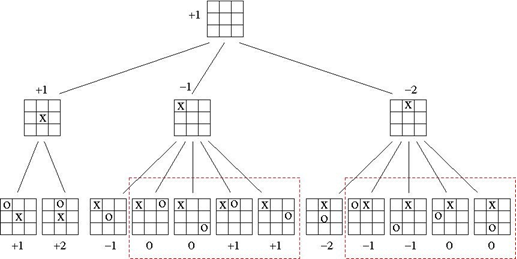
\includegraphics[width=\linewidth]{GameTree.png}
  \caption{Game Tree}
  \label{fig: Game_Tree}
\end{figure}

Figure \ref{fig: Game_Tree} shows a Game Tree.


\end{enumerate}
\section*{Problem 2}

\begin{enumerate}[label=(\alph*)]
  \item 
function AND-OR-GRAPH-SEARCH(problem) returns a conditional plan, or failure 
OR-SEARCH(problem.INITIAL-STATE, problem, [ ])
function OR-SEARCH(state, problem, path) returns a conditional plan, or failure
if problem.GOAL-TEST(state) then return the empty plan
if state is on path then return failure
for each action in problem.ACTIONS(state) do
plan AND-SEARCH(RESULTS(state, action), problem, [state | path])
if plan 6= failure then return [action | plan]
return failure
function AND-SEARCH(states, problem, path) returns a conditional plan, or failure
for each s(i) in states do:\\
plan(i) OR-SEARCH(s(i), problem, path)
if plan(i) = failure then return failure
return [if s1 then plan1
else if s2 then plan2
else if s(n1) then plan(n)1
else plan(n)]
\\\\
For slippery world, the graph shows corresponding conditions of going sucking one
or both the blocks in AND.For erratic world, the graph shows AND condition of stay-
ing back or moving to the next block.
\end{enumerate}
\end{document}
